Nous commencerons dans cette section par donner quelques définitions pour introduire la théorie des espaces de Teichmuller.

\begin{dfnt}{Espace de Teichmuller}
Soit $S$ une surface de genre $g$, un marquage de $S$ est un couple $(X,f)$ formé d'une surface de Riemann $X$ et d'un homéomorphisme préservant l'orientaion $f:S \to X$.
Sur l'ensemble des marquages de $S$, nous pouvons faire une relation d'équivalence $(X_1,f_1) \sim (X_2,f_2)$ si il existe $\alpha : X_1 \to X_2 $ tel que $f_2 \circ \alpha \circ f_1^{-1}$ soit un homéomorphisme de $S$ préservant l'orientation et isotope à l'identité.
L'espace des marquages quotienté par la relation s'appelle l'espace de Teichmuller et est noté $\mathbb{T}_g$
\end{dfnt}

\begin{rmq}
Si $g \geq 2$, pour toute courbe simple fermée $\alpha$ de $S$, il existe une unique géodésique fermée de $X$ librement isotope à $f(\alpha)$. Nous noterrons $L_{\alpha}(X)$ sa longeur hyperbolique et nous prenons la topologie la plus faible sur $T_g$ qui rendent ces fonctions continues.
\end{rmq}

\begin{dfnt}{Espace des modules}
On appele groupe modulaire le groupe des homéomorphisme préservant l'oriention de $S$ quotienté par ceux isotope à l'identité.Nous notterons ce groupe $Mod_g$.
Il agit de façon discrète sur $T_g$ et l'espace quotient est appelé espace des modules et est noté $\mathbb{M}_g$
\end{dfnt}

Il est naturel de ce demander à quoi ressemble ces espaces.

\begin{dfnt}{Dehn twist}
Soit $\gamma$ une courbe simple et fermée. Il existe un voisinage tubulaire de $\gamma$ noté $A$ homéomorphe à $[0;1] \times S^{1}$.
On définit le Dehn's twist comme l'homéomorphisme qui vaut l'indentité hors de $A$ et vaut $(t,s) \mapsto (t,e^{2i \pi t} s)$ sur $A$.
\end{dfnt}

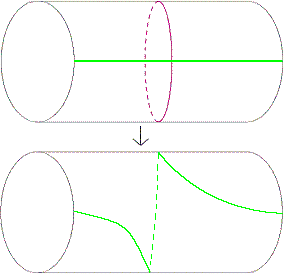
\includegraphics[width=6cm]{Image/Dehn_twist.png}

\begin{rmq}
Le théorème de Lickorisk affirme que le groupe modulaire est engendré par ces Dehn's twist et que plus précisément on peut choisir $2g+1$ générateurs \cite{Lickorish1964AFS}.
\end{rmq}

\begin{dfnt}{Feuilletage}
Un feuilletage mesuré est un feuilletage de la surface dont chaque arc porte une mesure. Ainsi la mesure d'un arc $\gamma$ ne dépent que de la feuille d'arrivé
\end{dfnt}

\begin{dfnt}{Lamination}
Une lamination est un ensemble fermé qui est un union (non nécessairement finie) de géodésiques.
Par chaque point x contenu dans $\lambda$ il ne passe que une seul géodésique.
Nous notterons cet espace $\mathbb{ML}(x)$
\end{dfnt}

\begin{dfnt}{Différentielle quadratique}
Une différentielle quadratique est une section du carré de l'espace tangeant canonique à X. Il s'écrit localement comme $\phi= \phi(z) dz^2$
\end{dfnt}

\begin{rmq}
Si $\phi(p) \neq 0$ on peut trouver une carte contenant $p$ dans laquel $\phi = dz^2$.
Ainsi $\phi$ détermine une métrique plate sur $X$ et un feuilletage $\mathbb{F}$ correspondant aux lignes horizontales.
\end{rmq}

Une différentielle quadratique est dite intégrable si \[
 \| \phi \| = \int_X | \phi | < \infty
\]
Nous notterons $\mathbb{Q}(x)$ l'espace de Banach des différentielles quadratiques intégrables.
%Differentiel quadratique
%Feuilletage
%Lamination
%tremblement de terre
%flot horocycle
%Nombre d'intersection
